\section{Structuration}
\sectitle{Structuration des données}

\begin{frame}
    \frametitle{Redondance des événements}
    Le constat :
    \begin{itemize}
        \item Événements redondants
        \item Informations dupliquées
    \end{itemize}
    \pause
    \vspace{2em}
    Notre choix :
    \begin{itemize}
        \item Événements fixes
        \item Nouvelle éditions chaque année
    \end{itemize}
\end{frame}

\begin{frame}
    \frametitle{Inexhaustion des formulaires}
    Le constat :
    \begin{itemize}
        \item Besoins spécifiques par événement
        \item Formulaires souvent similaires
    \end{itemize}
    \pause
    \vspace{2em}
    Notre choix :
    \begin{itemize}
        \item Formulaires personnalisables
        \item Construction récursive
    \end{itemize}
\end{frame}

\begin{frame}
    \frametitle{Gestion de la récurtion}
    Généralisation d'un formulaire $\Longrightarrow$ \textit{\textbf{FormWidget}} \\
    \pause
    \vspace{3em}
    3 types de \textit{FormWidget} :
    \begin{itemize}
        \item<3-> Natif
        \item<4-> Composite
        \item<5-> Liste
    \end{itemize}
\end{frame}

\begin{frame}
    \frametitle{Structure finale de la base de données}
    \begin{figure}
        \centering
        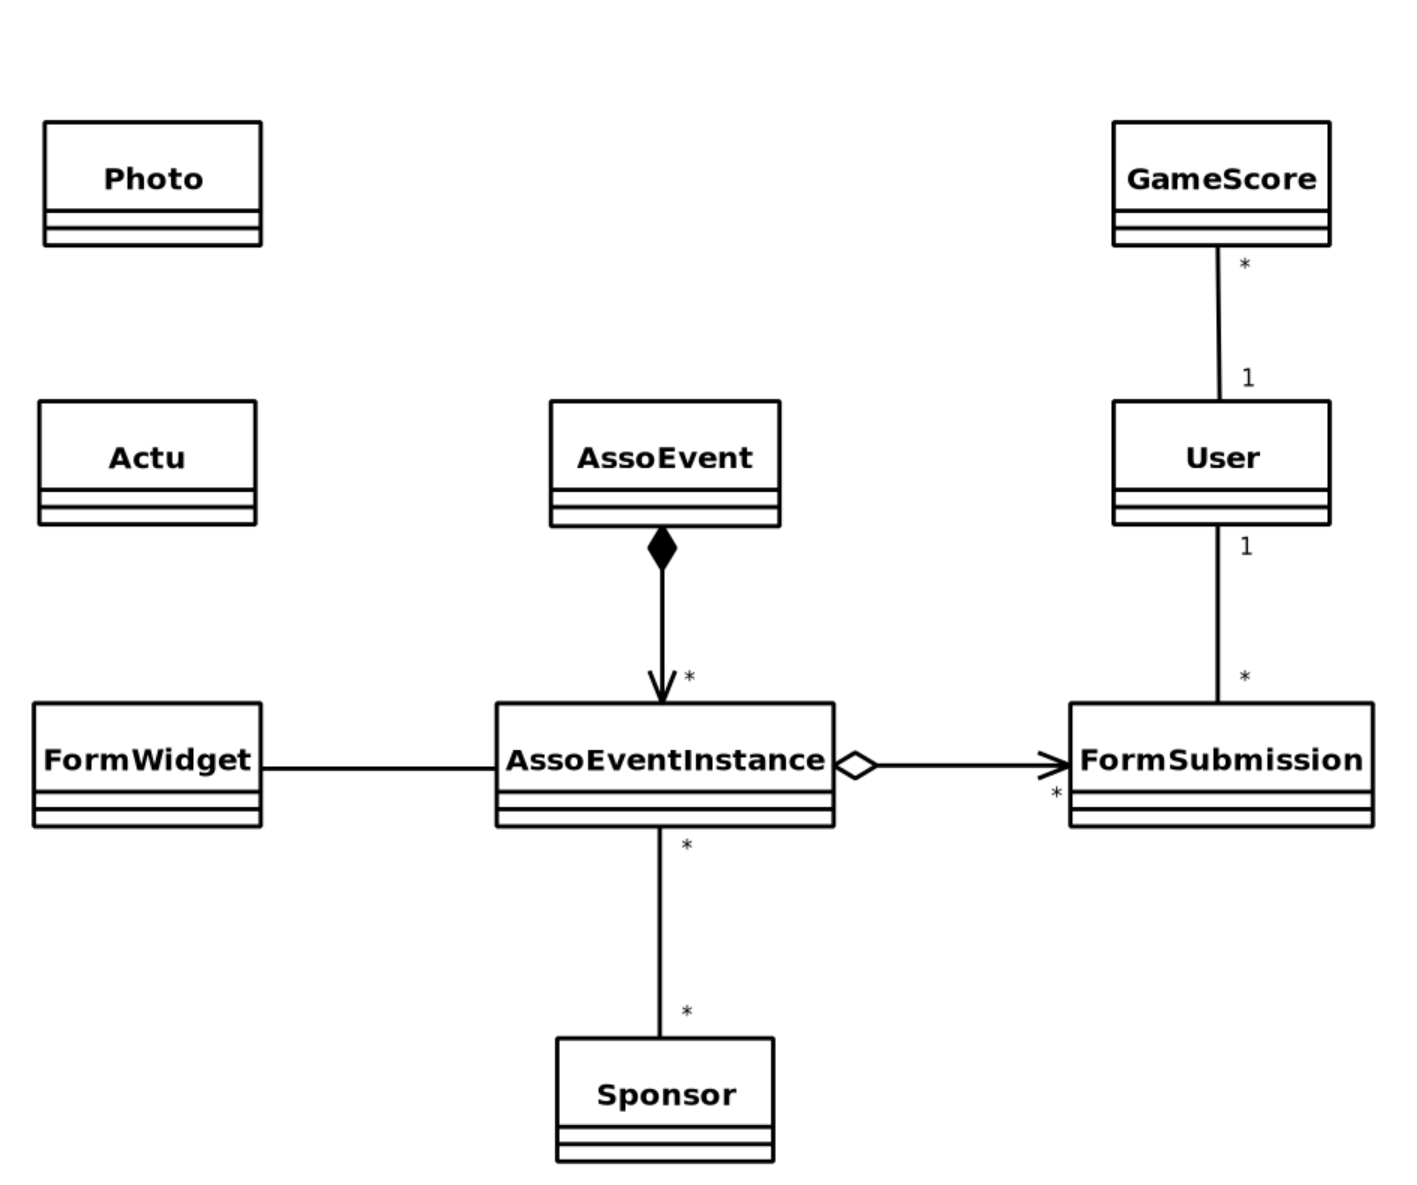
\includegraphics[width=0.8\textwidth]{pictures/database.png}
    \end{figure}
\end{frame}
